\documentclass[a4paper]{article}
\usepackage{a4wide}
\usepackage{amsmath}
  \DeclareMathOperator*{\argmax}{arg\,max}
  \newcommand\norm[1]{\left\lVert#1\right\rVert}
\usepackage{booktabs}
\usepackage{csquotes}
\usepackage{upquote}
\usepackage{float}
\usepackage{graphicx}
\usepackage{enumerate}
\usepackage{subcaption}
\usepackage{xcolor}


\title{Pattern and Speech Recognition WS2015-16 \\ Exercise 3}
\author{Atanas Poibrenski(2554135), Marimuthu Kalimuthu(2557695), Furkat Kochkarov(2557017)}

\begin{document}

\maketitle
\section*{Dimensionality Reduction}

\begin{enumerate}
	\item Linear classification - Iris dataset. \newline
	The data is linearly separable and the equation of the line is : \newline
	\textit{ax+b} where \textit{a=0.5 and b=-0.2}. \newline \newline
	This classification has no error since there are no misclassifications in the result. \newline
	
	\begin{figure}[H]
		\begin{center}
			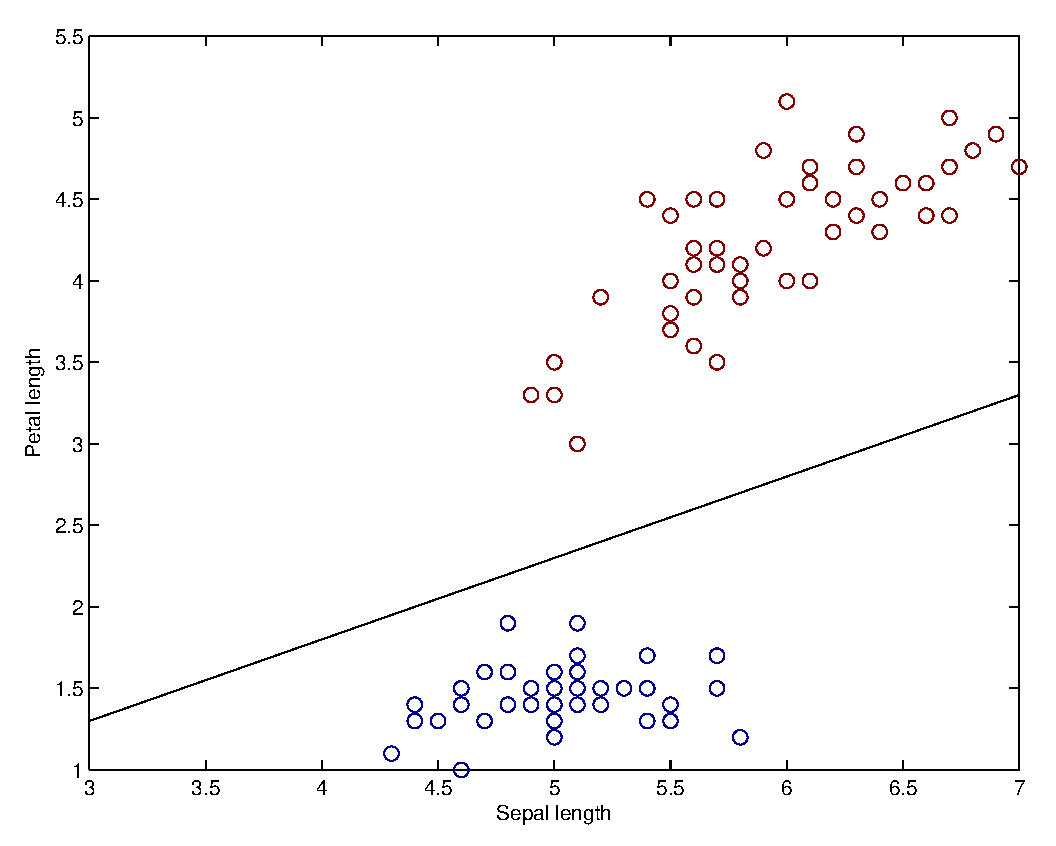
\includegraphics[width=0.85\textwidth]{Ex1.eps}
			\caption{linear classification}\label{fig:linclass}		
		\end{center}
	\end{figure}
	
\item The dimensions of W must be \textit{n by 1}. \newline \newline

\item \textbf{Grid search:} \newline \newline
 W = $\begin{bmatrix}
 	0.91 \\
 	0.51 
 \end{bmatrix}
 $ \newline \newline
See ``ex.m"

\item Plotting projection line

\begin{figure}[H]
	\begin{center}
		\includegraphics[width=0.85\textwidth]{Ex4.eps}
		\caption{Projection line}\label{fig:projline}		
	\end{center}
\end{figure}

	The line linearly separates the data and the equation of the line is : \newline
	\textit{ax+b} where \textit{a=0.91 and b=0.51}. \newline
	This is the line which reconstructs the data with least reconstruction error.

\item Projected data

\begin{figure}[H]
	\begin{center}
		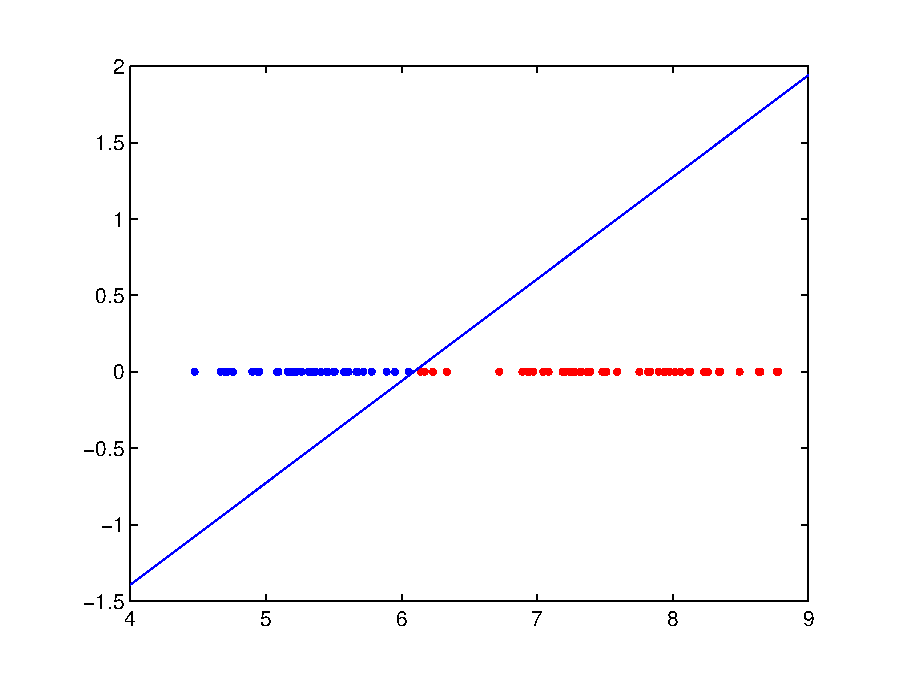
\includegraphics[width=0.85\textwidth]{Ex5.eps}
		\caption{Projected data}\label{fig:projdata}		
	\end{center}
\end{figure}

Yes the data is still linearly separable. And the equation of the line is : \newline
\textit{ax+b} where \textit{a=0.666 and b=-4.06}. \newline
And the misclassification(error) is zero.


\item \textit{(sepal length $|$ sepal width ) } projection
\begin{figure}[H]
	\begin{center}
		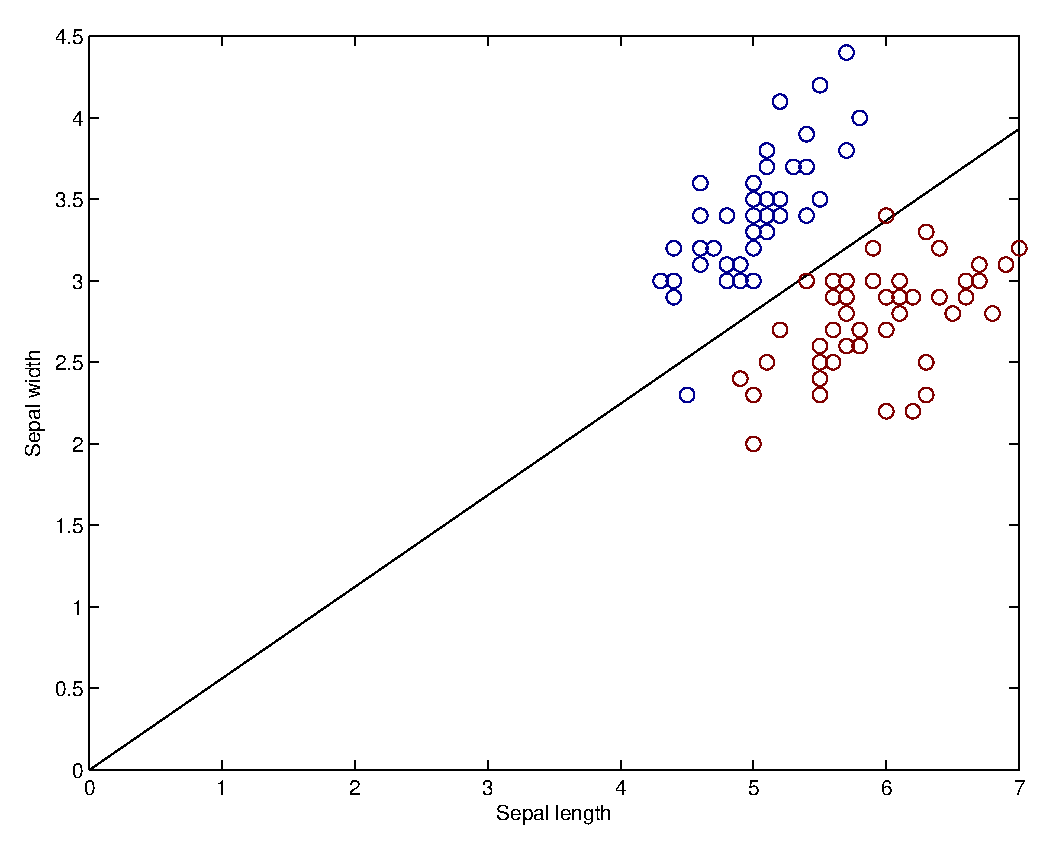
\includegraphics[width=0.67\textwidth]{Ex6_2.eps}
		\caption{(sepal length $|$ sepal width projection)}\label{fig:seplenwid}		
	\end{center}
\end{figure}

The error between the projected data and the original one,  (i.e.)
\begin{equation*}
\norm{ \biggl(\mathbf{X - \hat{X}}\biggr) }^2_2
\end{equation*}

is 31.97 \newline

The projection line does not separate the classes without error. This implies that this data cannot be projected into lower dimensional space and do linear separation without errors. \newline

Also, see \textit{``ex6.m"}


\begin{figure}[H]
	\begin{center}
		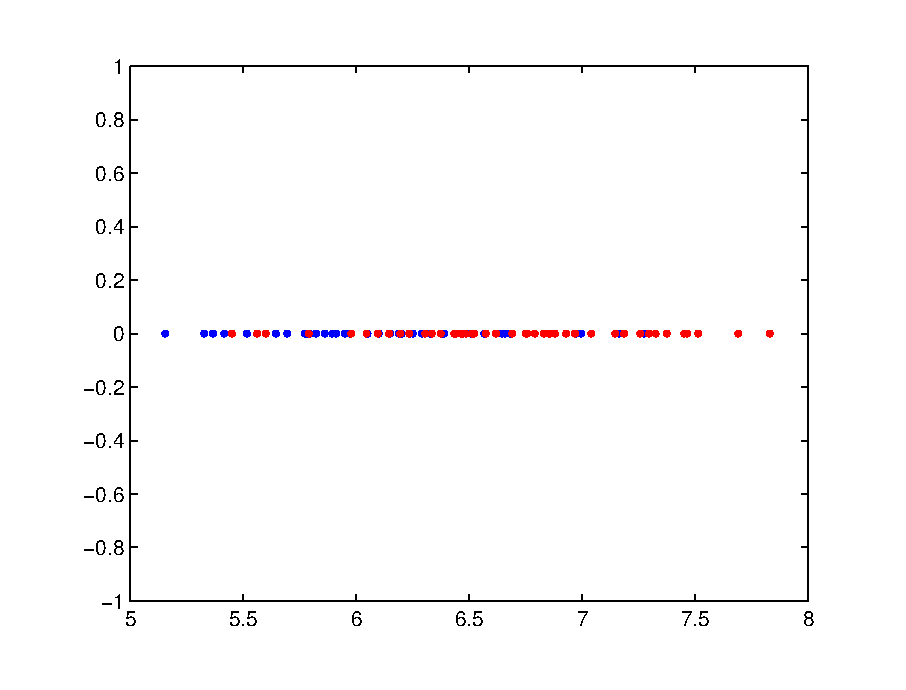
\includegraphics[width=0.67\textwidth]{Ex6_3.eps}
		\caption{(sepal length $|$ sepal width 1D-projection)}\label{fig:seplenwidproj}		
	\end{center}
\end{figure}

\end{enumerate}


\section*{Bonus}

Please see: ``bonus.m" \newline

\begin{enumerate}
	\item[] When we multiply the data by the transformation matrix `W' and compute the covariance matrix \textit{(i.e. matlab subtracts the mean from each element before calculating the covariance matrix)} of the result, we get the following \textit{4X4} matrix,

\begin{align*}
	\begin{bmatrix}
		2.767 &	6.094e-07 & -3.509e-07	& 6.855e-07 \\
		6.094e-07 & 0.228	& -7.534e-09 & -1.002e-07 \\
		-3.509e-07 & -7.534e-09 & 0.051	& 8.207e-09 \\
		6.855e-07 & -1.002e-07 & 8.207e-09 & 0.010 
	\end{bmatrix}
\end{align*}
	\newline
	
The covariance matrix of the 3D projection is the following \textit{3X3} matrix,

\begin{align*}
	\begin{bmatrix}
		2.767 &	6.094e-07 & -3.509e-07 \\
		6.094e-07 & 0.228	& -7.534e-09 \\
		-3.509e-07 & -7.534e-09 & 0.051 \\ 
	\end{bmatrix}
\end{align*}
\newline

The covariance matrix of the 2D projection is the following \textit{2X2} matrix,
\begin{align*}
	\begin{bmatrix}
		2.767 &	6.094e-07 \\
		6.094e-07 & 0.228 \\
	\end{bmatrix}
\end{align*}
\newline


The covariance matrix of the 1D projection is the following \textit{1X1} matrix,
\begin{align*}
	\begin{bmatrix}
		2.767 \\
	\end{bmatrix}
\end{align*}
\newline

Conclusion: Linear dimensionality reduction does not change the covariance/variance.

\end{enumerate}

\end{document}
